\documentclass{SciPress_2015}

%!!!!!!!!!!!!!!!!!!!!!!!!!!!!!!!!!!!!!!!!!!!!!!!!!!!!!!!!!!!!!!!!!!!!!
%---PLEASE USE XeLaTeX PACKAGE TO COMPILE THE TeX  FILE
%!!!!!!!!!!!!!!!!!!!!!!!!!!!!!!!!!!!!!!!!!!!!!!!!!!!!!!!!!!!!!!!!!!!!!

%--------------------------------------------- Basic packages (could be expanded by author)%
\usepackage{graphicx}
\usepackage{tabularx}
\usepackage{array}
\usepackage{makecell}
\usepackage{float}
\usepackage[intlimits]{amsmath}
\usepackage{amssymb}
\usepackage{exscale}
\usepackage{hyperref}
\usepackage{enumitem}
\usepackage{times}
%\usepackage{xparse}
\usepackage{fontspec}
\usepackage{subfigure}
\usepackage[usenames]{color}
%\usepackage{fontspec-patches}	
	% <-- DO NOT REMOVE this package,
				%       because the fonts (Times New Roman and Arial) will not be used in the document.
					% 	   If you don`t have this package, you can get it from the Internet or you can get this
					%       package from the archive The_Fontspec_package.zip which you downloaded with
					%       this current file.
%---------------------------------------------If you need include the .eps files, please uncomment the package bellow.%
%\usepackage{epsfig}
%--------------------------------------------- Override fonts to Times New Roman and Arial%
\renewcommand{\large}{\fontsize{14}{18pt}\selectfont}
\renewcommand{\small}{\fontsize{11}{13.6pt}\selectfont}
\setmainfont{Times New Roman}
\setsansfont{Arial}
%--------------------------------------------- New commands for quick editing of the document%
\newcommand{\titleformat}{\sffamily\bfseries \large}						%	<--- Doc. title
\newcommand{\authorformat}{\sffamily \large}							%	<--- Authors
\newcommand{\keywordsformat}{\noindent \small \sffamily}				%	<--- Kyewords
\newcommand{\abstractformat}{\noindent \textbf}						%	<--- Abstract
\newcommand{\contentformat}{\rmfamily \normalsize \vspace{18pt}}			%	<--- Main content
\newcommand{\email}{\sffamily \small \vspace{-8pt}}						%	<--- E-mail
\renewcommand{\subsection}{\textbf}	
%--------------------------------------------- Make all internal and external links - black color%
\hypersetup{
    colorlinks,%
    citecolor=black,%
    filecolor=black,%
    linkcolor=black,%
    urlcolor=black
}
%--------------------------------------------- Set the basic parameters of the page. DO NOT CHANGE!%
\special{papersize=210mm,297mm}
\textheight=25.6cm
%--------------------------------------------- For the Publisher to Enter:

\begin{document}

\title{\titleformat Number of Divisions by Two required for Collatz Cycles}
\author{\authorformat Christian Koch\inst{1}$^{,\rm{a{\rm{*}}}}$\textbf{,}
	Eldar Sultanow \inst{2}$^{,\rm{b}}$ and Sean Cox
\inst{3}$^{,\rm{c}}$}
\institute{\sffamily $^{\rm 1}$Technische Hochschule Nürnberg Georg Simon Ohm, Nuremberg, Germany\\
        \vspace{8pt} $^{\rm 2}$Capgemini, Nuremberg, Germany\\
        \vspace{8pt} $^{\rm 3}$RatPac-Dune Entertainment, Los Angeles, USA
}

\maketitle
\begin{center}
\vspace{2pt}\email{ $^{\rm a}$christian.koch@th-nuernberg.de,
	$^{\rm b}$eldar.sultanow@capgemini.com,
	$^{\rm c}$sean.cox@ratpacent.com}
\end{center}

\keywordsformat{{\textbf{Keywords:}Collatz Cycles, Divisions by Two, Cayley Graph, Free Group, Reachability}}

\contentformat
\abstractformat{Abstract.}
Using Data Science techniques, we identified empirically the number of divisions by two that are required for Collatz Cycles. We call this number cycle-alpha $\bar\alpha$. We provide a minimum and maximum condition for this cycle-alpha that must be proved in order to validate the correctness of this empirical finding. We prove the minimum condition for all $kx+1$ variants of Collatz sequences. We prove the maximum condition for special corner cases. The underlying idea is to represent the inverted Collatz sequence as a tree that consists of nodes labeled with odd Collatz sequence numbers. We do not claim to solve the \textit{Million Buck Problem}.

\section{Introduction}
\vspace{-6pt}
	
\hskip .5cm
Collatz introduced a surjective, non-injective function $g:\mathbb{N}\rightarrow\mathbb{N}$ as follows:

\begin{equation}
\label{eq:func_collatz}
g(m)=
\begin{cases}
3m+1	&	2\nmid m\\
m/2		&	\text{otherwise}
\end{cases}
\end{equation}

Let $(a_k)$ be a numerical sequence with $a_k=g^{(k)}(m)$, then a reversion produces an infinite number of sequences of reversely-written Collatz members \cite{Ref_Klisse}. Let $S$ be a set containing two elements $q$ and $r$, which are bijective functions over $\mathbb{Q}$: $q(x)=2x$ and $r(x)=\frac{1}{3}(x-1)$. Let a binary operation be the right-to-left composition of functions $q\circ r$, where $q\circ r(x)=q(r(x))$. The set, whose elements are all these compositions, forms a free group $F$ of rank 2 with respect to the free generating set $S$, where the identity element is the identity function $id_{\mathbb{Q}}=e$. The corresponding Cayley graph $Cay(F,S)=G$ is a regular tree \cite[p.~66]{Ref_Loeh}. We specify a subgraph $H$ of $G$ containing only vertices labeled by a string over alphabet $\{r,q\}$ without the inverses. This subgraph corresponds to the monoid $S^*$, which is freely generated by $S$. Let $Y^X=\{f\mid f\text{ is a map }X\rightarrow Y\}$ be the set of functions. We define the evaluation function $ev_{S^*}:S^*\times\{1\}\rightarrow\mathbb{Q}$ that evaluates an element of $S^*$, id est a composition of $q$ and $r$, for the given input value $1$. Furthermore we define the corestriction ${ev^0_{S^*}}$ of $ev_{S^*}$ to $\mathbb{N}$, which operates on a subset $T\subset S^*$ containing only those compositions of $q$ and $r$ that return a natural number when inputting the value $1$. Let $U\subset T$ be a subset of $T$, which does not contain a reduced word with two or more successive characters $r$. The corresponding tree $H_{U}\subset H_{T}$ reflects Collatz sequences. We define a tree $H_C$ by removing all even labeled vertices from $H_U$ via path contraction. A small section of the tree $H_C$ is shown in figure~\ref{fig:1}.

Let $v_1$ and $v_{n+1}$ be two vertices of $H_C$, where $v_1$ is reachable from $v_{n+1}$ with $level(v_1)-level(v_{n+1})=n$. Hence, a path $(v_{n+1},\ldots,v_1)$ exists between these two vertices. Theorem~\ref{theo:1} specifies the following relationship between $v_1$ and $v_{n+1}$.

\par\medskip
\begin{theorem}
	\label{theo:1}
	$l_{V(H_C)}(v_{n+1})=3^nl_{V(H_C)}(v_1)\prod_{i=1}^{n}\left(1+\frac{1}{3l_{V(H_C)}(v_{i})}\right)2^{-\alpha_i}$.
	In order to simplify readability, we waive writing down the vertex label function and put it shortly:\\
	$v_{n+1}=3^nv_1\prod_{i=1}^{n}\left(1+\frac{1}{3v_{i}}\right)2^{-\alpha_i}$.
	The value $\alpha_i\in\mathbb{N}$ is the number of divisions by two (the number of edges which have been contracted) between $v_i$ and $v_{i+1}$ in $H_U$.
\end{theorem}

In order to correctly determine successive nodes using theorem~\ref{theo:1}, we must consider the halting conditions. These are specified in Definition~\ref{def:halting_condition}.

\begin{definition}
	\label{def:halting_condition}
	When determining successive nodes starting at $v_1$ according to theorem~\ref{theo:1}, we halt if one of the following two conditions is fulfilled:
	\begin{enumerate}
		\item $v_{n+1}=1$
		\item $v_{n+1}\in\{v_1,v_2,\ldots,v_n\}$
	\end{enumerate}
	If the first condition applies, the Collatz conjecture is true for a specific sequence. When the second condition is fulfilled, the sequence has led to a cycle. For every starting node, except the root node (labeled with $1$), the Collatz conjecture is consequently falsified. Let us consider the example $v_1=13$, where the algorithm halts after two iterations, because the first condition is met:
	\[
	v_{n+1}=3^2\cdot\left(1+\frac{1}{3\cdot13}\right)\left(1+\frac{1}{3\cdot5}\right)\cdot2^{-7}=1
	\]
	
	If we examine the case $v_{1}=1$, we realize that the algorithm finishes after the first iteration, since both halting conditions are true. The sequence stops because the final node labeled with $1$ is reached. Furthermore, the sequence has led to a cycle:
	\[
	v_{n+1}=3\cdot\left(1+\frac{1}{3}\right)2^{-2}=1
	\]
	
	The trivial cycle is the only sequence where both conditions are fulfilled.
\end{definition}

\section{Collatz Cycles}
A path of length $n\geq 1$ that starts and ends at the same vertex, in which no vertex is repeated with the sole exception that the initial vertex is the terminal vertex, is called a cycle. A cycle of length $n$ is referred to as an $n$-cycle. When different nodes collapse on one, the graph is no longer necessarily a tree. Non-trivial cycles do not originate from the root, but cause the graph to be a disconnected graph.

Figure~\ref{fig:2} depicts a section of $H_{C,5}$, the $5x+1$ variant of $H_C$. Because of the two non-trivial cycles $43,17,27$ and $83,33,13$, in $H_{C,5}$ there does not exist a path between the root and the vertex $43$ and between the root and the vertex $83$. Utilizing the example of the graph $H_{C,5}$ we are able to deduct from the cycle $43,17,27$ the simple and self-evident equality $\textit{left-child}^3(43)=43$:
\begin{equation*}
\begin{array}{l}
\textit{left-child}(43)=\frac{1}{5}*\left(43*2^1-1\right)=17
\\[\medskipamount]
\textit{left-child}(17)=\frac{1}{5}*\left(17*2^3-1\right)=27
\\[\medskipamount]
\textit{left-child}(27)=\frac{1}{5}*\left(27*2^3-1\right)=43
\end{array}
\end{equation*}

Obviously, the authors note, it would be interesting to find out what circumstances enable a graph to have non-trivial cycles, whether it be the $5x+1$ variant of $H_C$, the $7x+1$ variant of $H_C$ or any variant of $H_C$; let us say the $kx+1$ variant of $H_C$ with $k\geq 1$.

Let us refer to a $kx+1$ variant of $H_C$ as $H_{C,k}$. By having introduced and proven theorem~\ref{theo:1} we already started an assertion about the reachability of successive nodes in $H_C$. This reachability relationship can be generalized for any graph $H_{C,k}$ as follows:
\begin{equation}
\label{eq:generalized_reachability}
v_{n+1}=k^nv_1\prod_{i=1}^{n}\left(1+\frac{1}{kv_{i}}\right)2^{-\alpha_i}
\end{equation}

This generalization leads to the condition for an existence of an $n$-cycle in any $kx+1$ variant of $H_C$, which looks analogous to the condition given by equation~\ref{eq:func_cycle} that specifies $H_C$ has a cycle:
\begin{equation}
\label{eq:generalized_cycle}
2^\alpha=\prod_{i=1}^{n}\left(k+\frac{1}{v_i}\right)
\end{equation}

The natural number $\alpha$ is the sum of edges that have been contracted between the vertices $v_i$ forming the cycle, in other words $\alpha$ is the number of divisions by $2$ within the sequence. The natural number $n$ is the cycle length and $k$ obviously specifies the variant of $H_C$. Since between each vertex at least one edge has been contracted (at least one division by $2$ took place), we know that our exponent alpha is greater than or equal to the sequence length:
\begin{equation}
\label{eq:n_alpha}
\alpha\ge n
\end{equation}

\par\medskip
Using incremental search, one can calculate cycles through trial and error. Table~\ref{table:known_cycles} lists all empirically discovered cycles having a length up to $100$ that appear in $kx+1$ variants of $H_C$ for $k\in[1,1000]$. Within each of these variants, the cycles have been searched at potential starting nodes $v_1$ with a label between $1$ and $1000$. Note that the cycles in table~\ref{table:known_cycles} are written in reverse order, i.e. in the order which corresponds to the Collatz sequence. To obtain the cycles in terms of graph theory referring to the graph $H_C$, read them from right to left.

\begin{table}[H]
	\centering
	\begin{tabular}{|l|r|r|c|}
		\hline
		\thead{k} &
		\thead{\textbf{cycle}} &
		\thead{$\alpha$} &
		\thead{\textbf{non-trivial}} \\
		\hline
		1 &
		1 &
		1 &
		\\
		\hline
		3 &
		1 &
		2 &
		\\
		\hline
		5 &
		1,3 &
		5 &
		\\
		\hline
		5 &
		13,33,83 &
		7 &
		\checkmark \\
		\hline
		5 &
		27,17,43 &
		7 &
		\checkmark \\
		\hline
		7 &
		1 &
		3 &
		\\
		\hline
		15 &
		1 &
		4 &
		\\
		\hline
		31 &
		1 &
		5 &
		\\
		\hline
		63 &
		1 &
		6 &
		\\
		\hline
		127 &
		1 &
		7 &
		\\
		\hline
		181 &
		27,611 &
		15 &
		\checkmark \\
		\hline
		181 &
		35,99 &
		15 &
		\checkmark \\
		\hline
		255 &
		1 &
		8 &
		\\
		\hline
		511 &
		1 &
		9 &
		\\
		\hline
	\end{tabular}
	\caption{Known $n$-cycles in $kx+1$ variants of $H_C$ for $k\leq1000$, $n\leq 100$}
	\label{table:known_cycles}
\end{table}

Based on the results shown in table~\ref{table:known_cycles} we state the following theorem~\ref{theo:2} that renders more precisely the prerequisite for cycles that may occur in variants of $H_C$.

\par\medskip
\begin{theorem}
	\label{theo:2}
	An $n$-cycle can only exist in a graph $H_{C,k}$, that means in a $kx+1$ variant of $H_C$, if the following equation holds:
	\begin{equation*}
	2^{\bar\alpha}=2^{\lfloor n\log_2k\rfloor+1}=\prod_{i=1}^{n}\left(k+\frac{1}{v_i}\right)
	\end{equation*}
\end{theorem}

\par\medskip
The key of theorem~\ref{theo:2} consists in the claim that, in order for an $n$-cycle to occur, the exponent $\alpha$ has to be $\bar\alpha=\lfloor n\log_2k\rfloor+1$. We approach a proof by expressing formally that $\bar\alpha$ is not allowed to be smaller and it is not allowed to be greater than $\lfloor n\log_2k\rfloor+1$, in other words we indicate a lower and an upper limit for $\bar\alpha$ as follows:

\begin{samepage}
	\begin{flalign}
	\label{eq:inequality_min}
	&\bar\alpha>\lfloor n\log_2k\rfloor\\	
	\label{eq:inequality_max}
	&\bar\alpha<\lfloor n\log_2k\rfloor+2
	\end{flalign}
\end{samepage}

The validity of the first part (\ref{eq:inequality_min}), which specifies $\lfloor n\log_2k\rfloor+1$ as the lower limit for $\bar\alpha$, can be demonstrated in a fairly simple way: Our starting point is equation~\ref{eq:generalized_reachability}, which describes the relationship of successive vertices in $H_{C,k}$. Having a cycle, requires us to consider the first and the last vertex being one and the same $v_{n+1}=v_1$. Setting a smaller exponent $\bar\alpha=\lfloor n\log_2k\rfloor$ into equation~\ref{eq:generalized_reachability} results in the inequality $v_{n+1}>v_1$, which is in any case a true statement:
\begin{equation*}
\begin{array}{l}
k^nv_12^{-\lfloor n\log_2k\rfloor}\prod_{i=1}^{n}\left(1+\frac{1}{kv_{i}}\right)>v_1
\\[\medskipamount]
k^n\prod_{i=1}^{n}\left(1+\frac{1}{kv_{i}}\right)>2^{\lfloor\ nlog_2k\rfloor}
\\[\medskipamount]
\log_2\left(k^n\prod_{i=1}^{n}\left(1+\frac{1}{kv_{i}}\right)\right)>\lfloor n\log_2k\rfloor
\\[\medskipamount]
n\log_2k+log_2\left(\prod_{i=1}^{n}\left(1+\frac{1}{kv_{i}}\right)\right)>\lfloor n\log_2k\rfloor
\end{array}	
\end{equation*}

The validity of the second part (\ref{eq:inequality_max}) is not so trivial to prove. Analogous to the above-shown proof of the cylce-alpha's lower limit, we again refer to equation~\ref{eq:generalized_reachability} as our starting point and we need to show that $v_{n+1}$ is smaller than $v_1$ if $\alpha=\lfloor\ nlog_2k\rfloor+2$:
\begin{equation*}
\begin{array}{l}
k^nv_12^{-\left(\lfloor n\log_2k\rfloor+2\right)}\prod_{i=1}^{n}\left(1+\frac{1}{kv_{i}}\right)<v_1
\\[\medskipamount]
k^n\prod_{i=1}^{n}\left(1+\frac{1}{kv_{i}}\right)<2^{\left(\lfloor n\log_2k\rfloor+2\right)}
\end{array}	
\end{equation*}
This leads to the following general condition for the validity of the cycle-alpha's upper limit:
\begin{equation}
\label{eq:condition_max}
n\log_2k-\lfloor n\log_2k\rfloor<2-log_2\left(\prod_{i=1}^{n}\left(1+\frac{1}{kv_{i}}\right)\right)
\end{equation}

A product $\prod(1+a_n)$ with positive terms $a_n$ is convergent if the series $\sum a_n$ converges, see Knopp \cite[p.~220]{Ref_Knopp}. Thus, to verify whether the product in condition~\ref{eq:condition_max} is converging towards a limiting value, it is sufficient to examine the following sum:
\begin{equation*}
\sum_{i=1}^{n}\frac{1}{kv_{i}}
\end{equation*}

\begin{figure}
	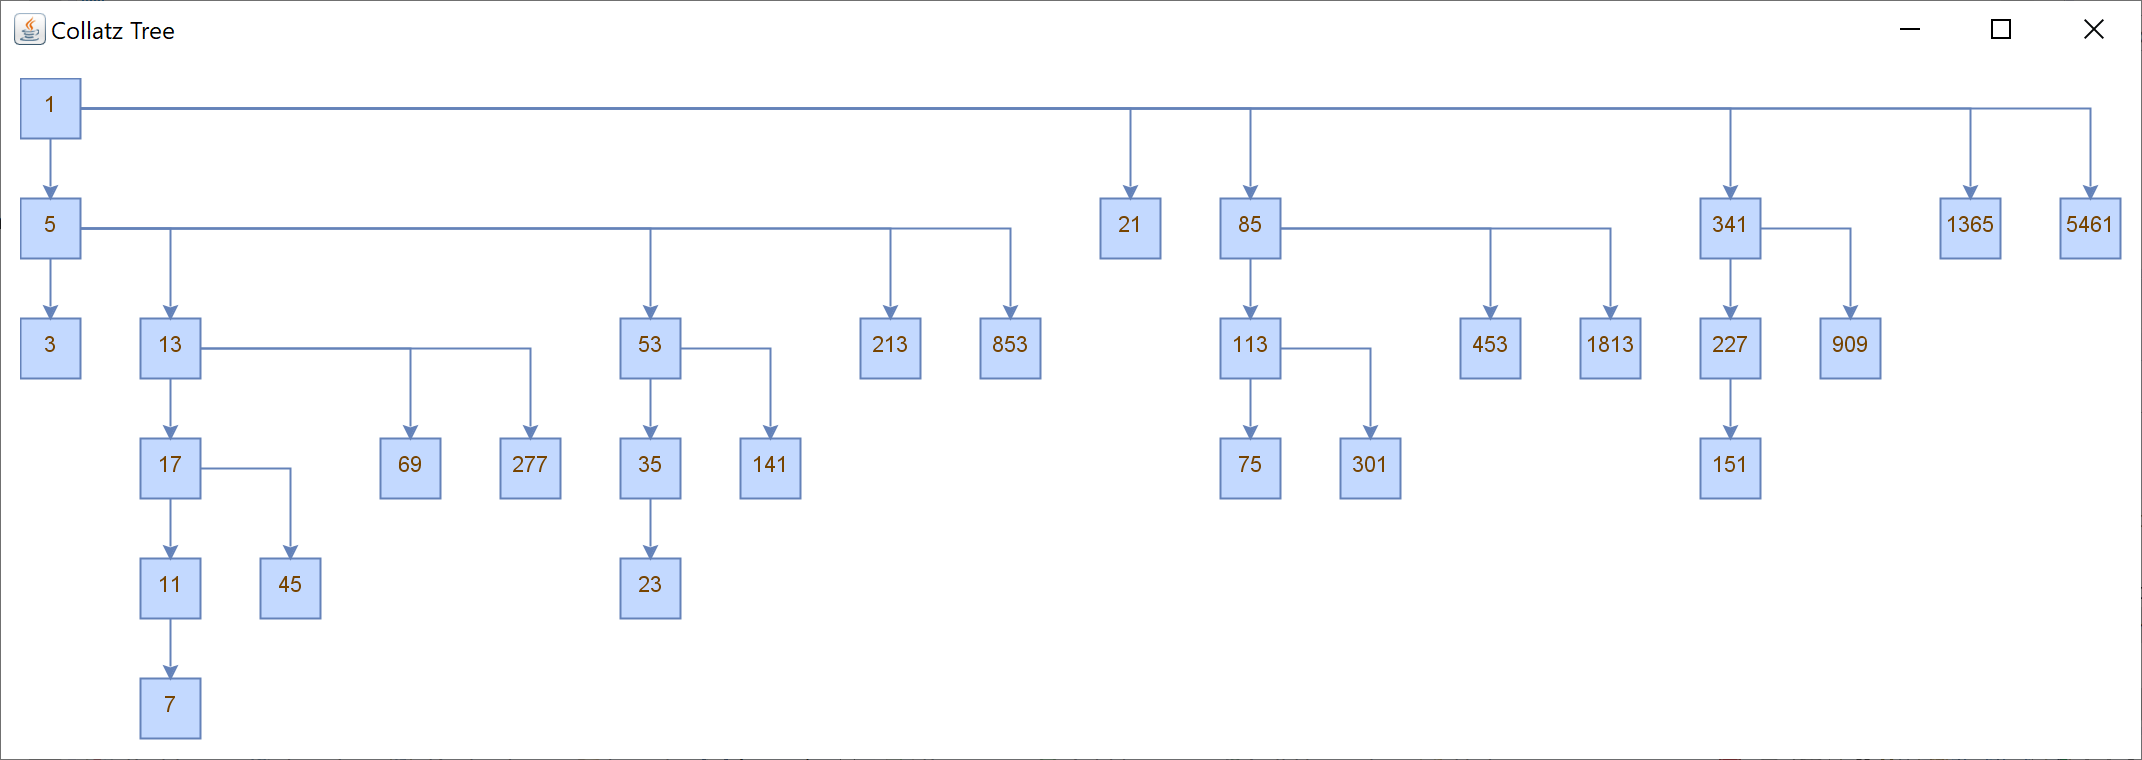
\includegraphics[width=1.00\textwidth]{figures/h_c.png}
	\caption{Small section of $H_C$}
	\label{fig:1}
\end{figure}

\begin{figure}
	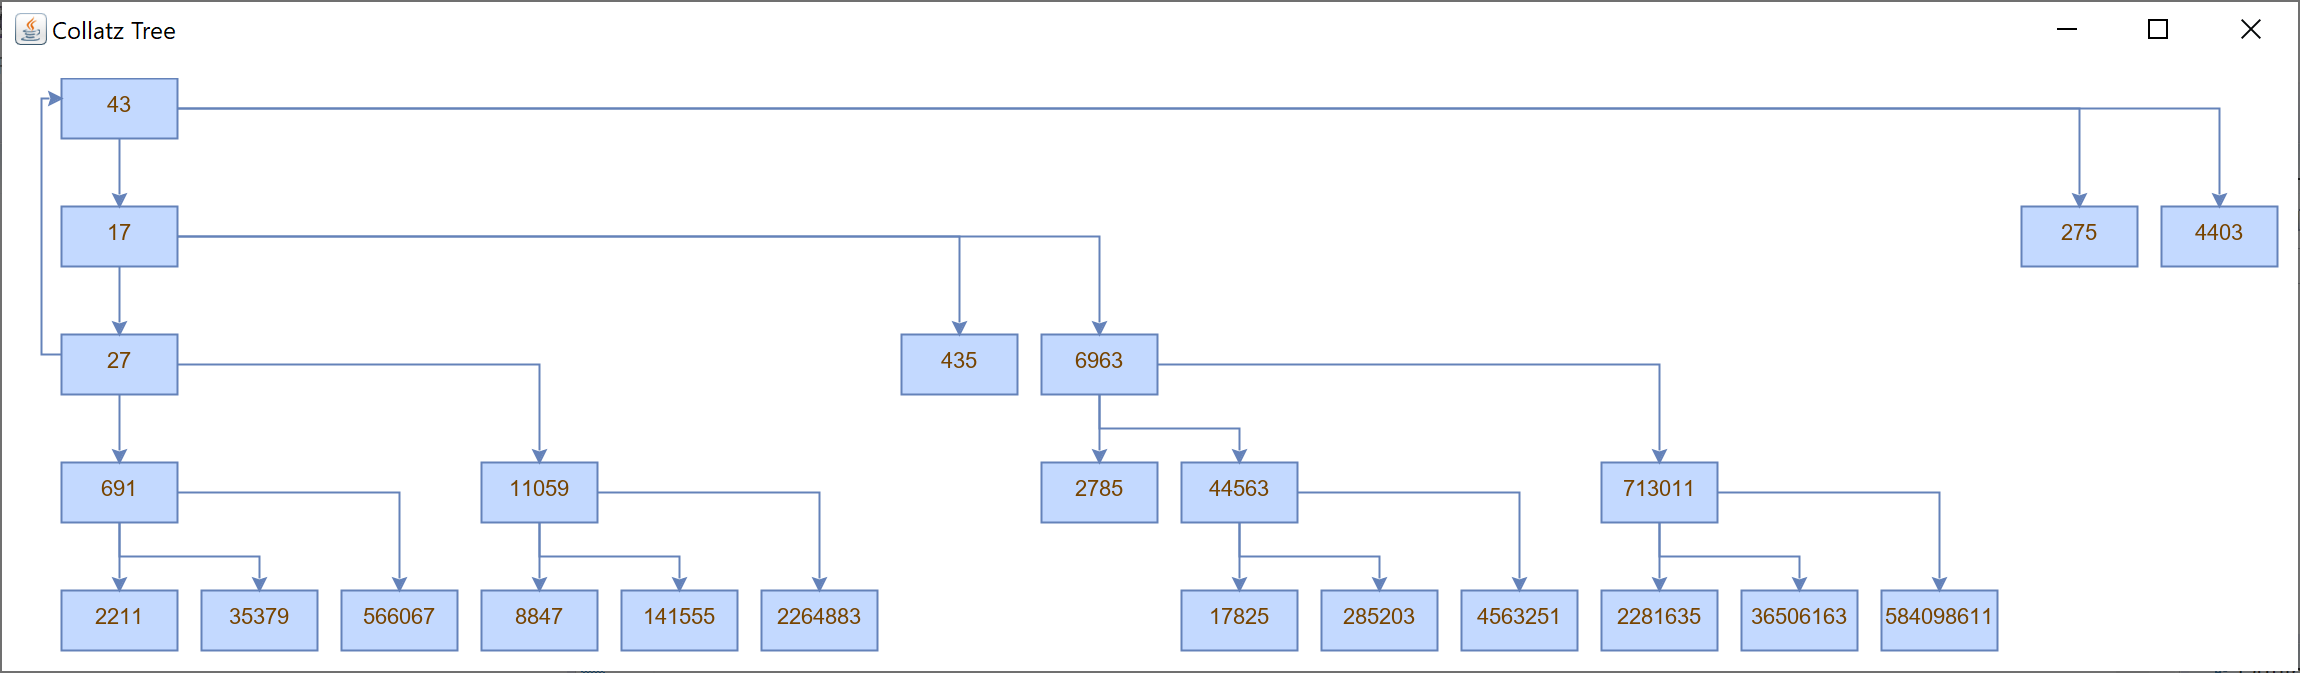
\includegraphics[width=1.00\textwidth]{figures/h_c5a.png}
	\caption{Section of $H_{C,5}$ including the $3$-cycle $43,17,27$}
	\label{fig:2}
\end{figure}

\section{Conclusion and outlook}
We defined an algebraic graph structure that expresses the Collatz sequences in the form of a tree. Next, the vertex reachability properties were unveiled by examining the relationship between successive nodes in $H_C$. Moreover, we dealt with graphs that represent other variants of Collatz sequences, for instance $5x+1$ or $181x+1$. The interesting part of both variants just mentioned is that for these sequences the existence of cycles is known. With regard to a proof of the Collatz conjecture, theorem~\ref{theo:2} seem promising. They serve as the basis for further investigations of the problem.


\begin{thebibliography}{99}

\bibitem{Ref_Klisse}
M. Klisse, Das Collatz-Problem: L\"osungs- und Erkl\"arungsans\"atze f\"ur 
die 1937 von Lothar Collatz entdeckte (3n+1)-Vermutung. (2010)

\bibitem{Ref_Loeh}
C. Löh, Geometric Group Theory: An Introduction. Springer, 2010, DOI
https://doi.org/10.1007/978-3-319-72254-2

\bibitem{Ref_Bondy_Murty}
J. A. Bondy and U. S. R. Murty: Graph Theory with Applications. Elsevier
Science, 1976, ISBN 0-444-19451-7

\bibitem{Ref_Bonnington_Little}
C. P. Bonnington and C. H.C. Little: The Foundations of Topological
Graph Theory. Springer, 1995, DOl: 10.1007/978-1-4612-2540-9

\bibitem{Ref_Bender_Williamson}
E. A. Bender and S. G. Williamson: Mathematics for Algorithm and System
Analysis. Dover, 2005, ISBN 0-486-44250-0.

\bibitem{Ref_Truemper}
M. Tr\"umper: The Collatz Problem in the Light of an Infinite Free
Semigroup. Chinese Journal of Mathematics, Volume 2014, DOI:
http://dx.doi.org/10.1155/2014/756917

\bibitem{Ref_Almeida}
J. Almeida: Profinite semigroups and applications. In V. B. Kudryavtsev
and I. G. Rosenberg (eds.), Structural Theory of Automata, Semigroups,
and Universal Algebra. Springer, 2005.

\bibitem{Ref_Johnsonbaugh}
R. Johnsonbaugh: Discrete Mathematics (Eighth Edition).
Pearson, 2017, ISBN 0-321-96468-3.

\bibitem{Ref_MacLane_Birkhoff}
S. Mac Lane and G. Birkhoff: Algebra (Third Edition). AMS Chelsea
Publishing, 1999, ISBN 0821816462.

\bibitem{Ref_Novak_etal}
V. Novák, I. Perfilieva, and J. Močkoř: Mathematical Principles of
Fuzzy Logic. Springer, 1999, DOI 10.1007/978-1-4615-5217-8

\bibitem{Ref_Pellissier}
R. Angot-Pellissier: The Relation Between Logic, Set Theory and Topos
Theory as It Is Used by Alain Badiou. In A. Koslow and A. Buchsbaum
(eds.), The Road to Universal Logic: Festschrift for the 50th Birthday
of Jean-Yves Beziau (Volume II). Birkhäuser, 2015,
DOI 10.1007/978-3-319-15368-1

\bibitem{Ref_Helemskii}
A. Ya. Helemskii: Lectures and Exercises on Functional Analysis.
American Mathematical Society, 2006, ISBN 0-8218-4098-3

\bibitem{Ref_Rosen}
K. H. Rosen: Discrete Mathematics and Its Applications (Seventh Edition).
McGraw-Hill, 2011, ISBN 978-0-07-338309-5

\bibitem{Ref_Makinson}
D. Makinson: Sets, Logic and Maths for Computing (Second Edition).
Springer, 2012, DOI 10.1007/978-1-4471-2500-6

\bibitem{Ref_Korte_Vygen}
B. Korte and J. Vygen: Combinatorial Optimization: Theory and Algorithms
(Sixth Edition). Springer, 2018,
DOI https://doi.org/10.1007/978-3-662-56039-6

\bibitem{Ref_Mehlhorn_Sanders}
K. Mehlhorn and P. Sanders: Algorithms and Data Structures: The Basic
Toolbox. Springer, 2008, DOI 10.1007/978-3-540-77978-0

\bibitem{Ref_Du_Ko_Hu}
D.-Z. Du, K.-I Ko, and Z. Hu: Design and Analysis of Approximation
Algorithms. Springer, 2012, DOI 10.1007/978-1-4614-1701-9

\bibitem{Ref_Ehrig_etal}
H. Ehrig, K. Ehrig, U. Prange, and G. Taentzer: Fundamentals
of Algebraic Graph Transformation. Springer, 2006,
DOI 10.1007/3-540-31188-2

\bibitem{Ref_Childs}
L. N. Childs: A Concrete Introduction to Higher Algebra (Third Edition). 
Springer, 2006, DOI 10.1007/978-0-387-74725-5

\bibitem{Ref_Voloshin}
V. I. Voloshin: Introduction to Graph and Hypergraph Theory.
Nova Science Publishers, 2011, ISBN 978-1-61470-112-5

\bibitem{Ref_Loehr}
N. A. Loehr: Combinatorics (Second Edition).
CRC Press, 2017, ISBN 978-1-4987-8025-4

\bibitem{Ref_Conrow}
K. Conrow: The Structure of the Collatz Graph; A Recursive Production
of the Predecessor Tree; Proof of the Collatz 3x+1 Conjecture.
http://citeseerx.ist.psu.edu/viewdoc/summary?doi=10.1.1.423.3396

\bibitem{Ref_Bauer}
F. L. Bauer: Historische Notizen zur Informatik.
Springer, 2009, DOI 10.1007/978-3-540-85790-7

\bibitem{Ref_Hercher}
C. Hercher: Über die Länge nicht-trivialer Collatz-Zyklen.
Die Wurzel, Hefte 6 und 7/2018 

\end{thebibliography}


\end{document} 